\subsection{Sous-mission B3}

	\begin{vwcol}[widths={0.65,0.2}, rule=0pt]
	\begin{minipage}{0.7\textwidth}
	\paragraph{Objectifs de la mission}

	Mettre en valeur les 4 étapes de températures à la surface de la planète. 
	\end{minipage}

	\begin{minipage}{0.25\textwidth}
	\begin{flushright}
	\paragraph{Techniques utilisées}
	
	Seuillage avancé \& Addition
	\end{flushright}
	\end{minipage}

	\end{vwcol} 

	\begin{figure}[h]
	\centering
		\begin{multicols}{2}
		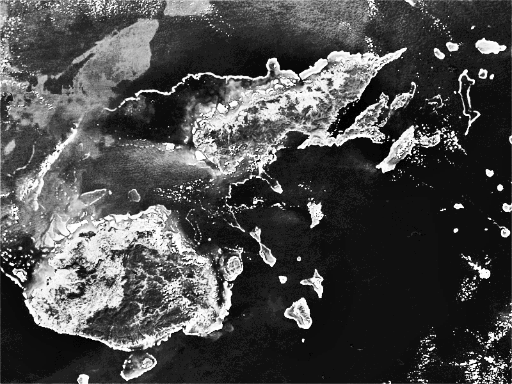
\includegraphics[scale=0.55]{images/HD215497.png}
		Avant

		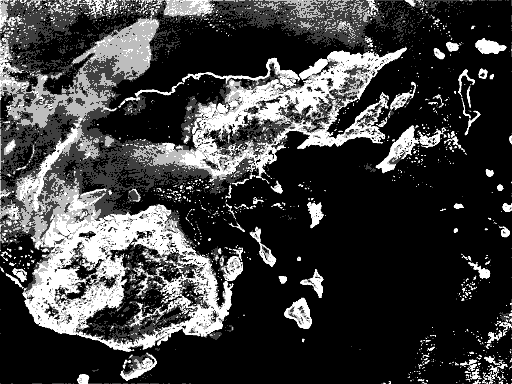
\includegraphics[scale=0.55]{images/MissionB3.png}
		Après
		\end{multicols}
	\end{figure}
	\vspace{-0.9cm}

	\paragraph{Procédé}	
		Nous avons choisi de mettre en avant les différentes étapes de thempératures par des plages de couleur spécifiques. Pour se faire nous avons effectué un \emph{seuillage avancé} individuel pour chaque plages de température. Nous avons ensuite effectué une \emph{addition} de chacun des résultats pour obtenir l'image finale. 